\documentclass[12pt]{article}

\usepackage[portuguese]{babel}
\usepackage{graphicx}
\usepackage[section]{placeins}
\usepackage{float}
\usepackage{url}

\graphicspath{ {figures} }

\author{João Vitor Maia Neves Cordeiro}
\title{Segundo trabalho prático: Wireshark e SNMP}
\date{\today}

\addto\captionsportuguese{\renewcommand*\contentsname{Sumário}}

\begin{document}

\maketitle

\begin{abstract}
O presente trabalho visa demonstrar a utilização de ferramentas de gerenciamento de rede como o PRTG e o Wireshark, a fim de dar ao leitor o material necessário para compreender o uso desses softwares e replicar os experimentos realizados. Com o uso dos programas foi realizado um monitoramento que inicialmente seria de 3 dias com interrupções, mas com o professor oferecendo uma extensão do prazo, foi decidido por continuar o monitoramento durante uma semana. Durante o monitoramento foram compreendidos conceitos importantes sobre os protocolos utilizados como ARP, SNMP e UDP; Além disso, essa atividade também proporcionou um entendimento de como gerenciar uma rede doméstica, verificando a eficiência da rede.
\end{abstract}

\tableofcontents

\section{Introdução}

O monitoramento de rede é de suma importância quando discutimos sobre Quality of Service (QoS) e segurança preventiva contra ataques cibernéticos. Nesse relatório será demonstrado o trabalho prático realizado utilizando as ferramentas PRTG e Wireshark, um monitoramento detalhado para nos ajudar a compreender o tráfego de pacotes entre os dispositivos de uma rede doméstica. As ferramentas utilizadas são renomadas e tidas como padrões do mercado (apesar de existirem outras boas ferramentas disponíveis), portanto o compreendimento da utilização delas é imprescindível para um profissional da computação que deseje trabalhar com redes de computadores.

\section{Ferramentas utilizadas}

\subsection{PRTG}

O PRTG Network Monitor é uma ferramenta \emph{agentless} de monitoramento de rede, ou seja, a instalação é feita em um computador central e os outros computadores da rede não precisam instalar agentes próprios. Além disso, o software conta com uma interface \emph{web-based} moderna e com boa usabilidade que permite gerar relatórios e gráficos em cima das medições realizadas. Como pontos negativos do software pode-se dizer que ele é restrito à plataforma Windows, além de que por se tratar de um software proprietário com um \emph{trial} de 30 dias o acesos a ele é mais restrito do que a suas alternativas open-source.

\subsection{Wireshark}

O Wireshark é uma ferramenta \emph{open souce} e gratuita para monitoramento de pacotes que nos permite verificar a entrada e saída de dados do computador. Diferentemente do PRTG, ele possui suporte para diversas plataformas e todos os recursos estão disponíveis de forma gratuita.

\section{Topologia da rede}

O monitoramento foi realizado em uma rede doméstica, utilizando os serviços da CLARO S/A, tendo conectados nas redes os seguintes dispositivos: um Desktop customizado, um Macbook Air 2017 e um notebook Lenovo S30. O PRTG Server Core foi instalado no Desktop, devido a maior robustez dessa máquina, os outros dispositivos foram adicionados ao monitoramento pelo painel do PRTG. Entretanto, não foi possível adicionar sensores muito complexos aos outros dispositivos da rede. Todos os dispositivos foram utilizados na análise do Wireshark.

\begin{figure}[H]
    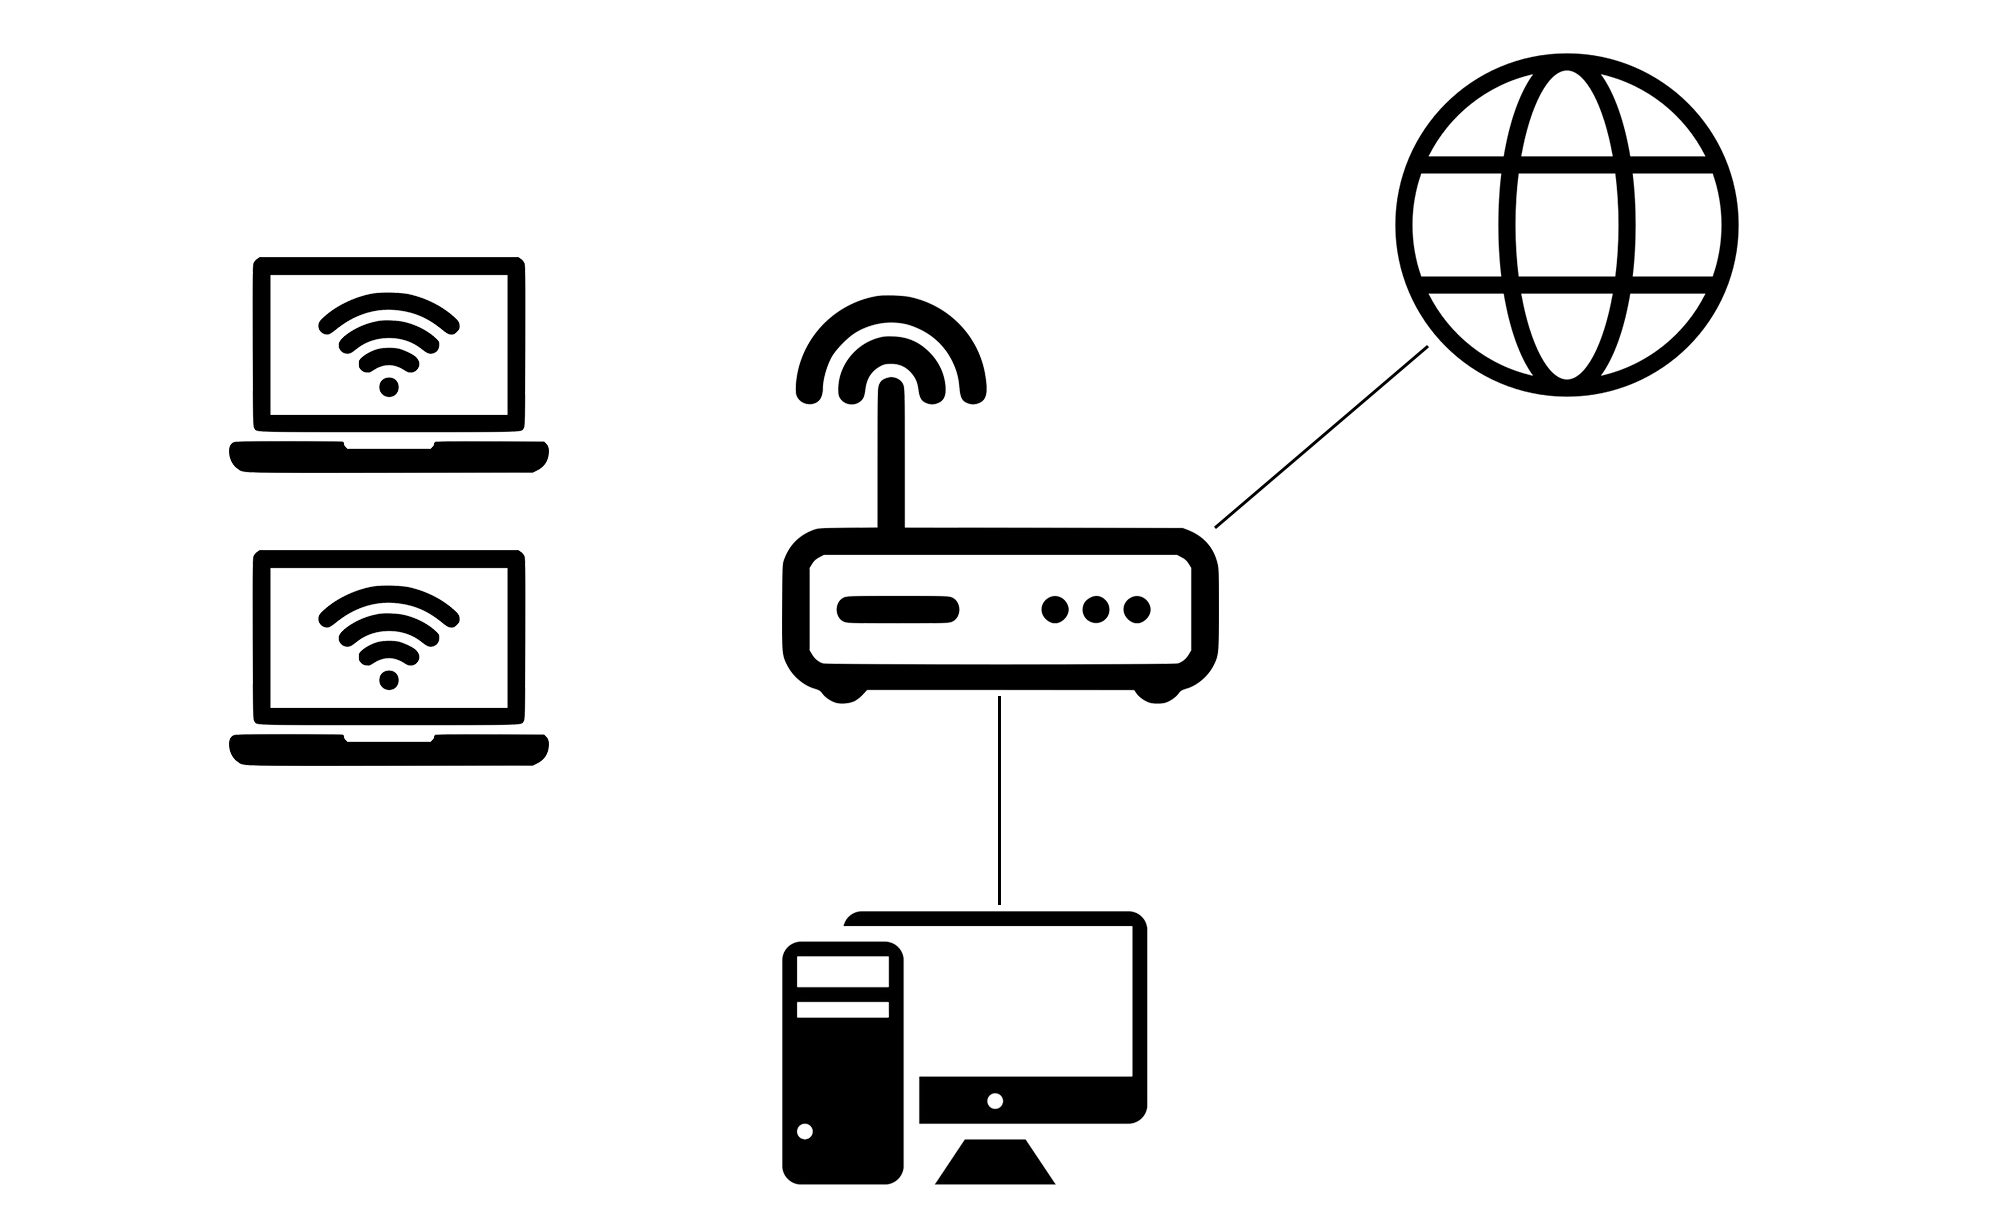
\includegraphics[width=\linewidth]{topology.png}
    \caption{Uma rede doméstica com 4 dispositivos: Um notebook Lenovo (192.168.0.102), um macbook air (192.168.0.101), um desktop gamer (192.168.0.100) e um Modem com roteador (192.168.1.1)}
\end{figure}

\subsection{Equipamentos}

\begin{itemize}
    \item Desktop
    \begin{itemize}
        \item Processador: Ryzen 5 3600 @ 3.60 GHz
        \item Memória RAM: 16GB DDR4 3000Mhz
        \item Sistema Operacional: Windows 10
        \item Adaptador Ethernet: Realtek PCIe GBE Family Controller
    \end{itemize}
    \item Macbook
    \begin{itemize}
        \item Processador: Intel i5 3600 @ 3.60 GHz
        \item Memória RAM: 8 GB LPDDR3 1600 MHz
        \item Sistema Operacional: OSX Mojave
        \item Adaptador Wireless: 802.11ac
    \end{itemize}
    \item Notebook Lenovo S30
    \begin{itemize}
        \item Processador: Intel® Core™ i5-1035G1 Quad Core 1.0 GHz com Turbo Max até 3.6 GHz
        \item Memória RAM: 4 GB DDR4 2666 MHz + 16 GB Optane (4 GB soldado + 1 slot livre)
        \item Sistema Operacional: Windows 10
        \item Adaptador Wireless: 802.11ac
    \end{itemize}
    \item Modem
    \begin{itemize}
        \item Modelo: TP-Link WR740N
        \item Frequência: 2.4 GHz
    \end{itemize}
\end{itemize}

\section{Monitoramento}

O PRTG diferencia os dispostivos entre \emph{Probe device} e \emph{network device}, sendo que o primeiro diz respeito a dispositivos que possuem o PRTG Core Server instalado diretamente, possibilitando melhores medições com sensores mais avançados. Enquanto o segundo são os dispositivos conectados na rede e visualizados através de protocolos de rede apenas. Durante esse trabalho foi utilizado apenas um \emph{probe device} devido a impossibilidade de instalar outros na rede, tendo em vista que o PRTG é instalável apenas no Windows e os outros computadores da rede utilizam sistemas Unix.

\subsection{Probe health}

\begin{figure}[H]
    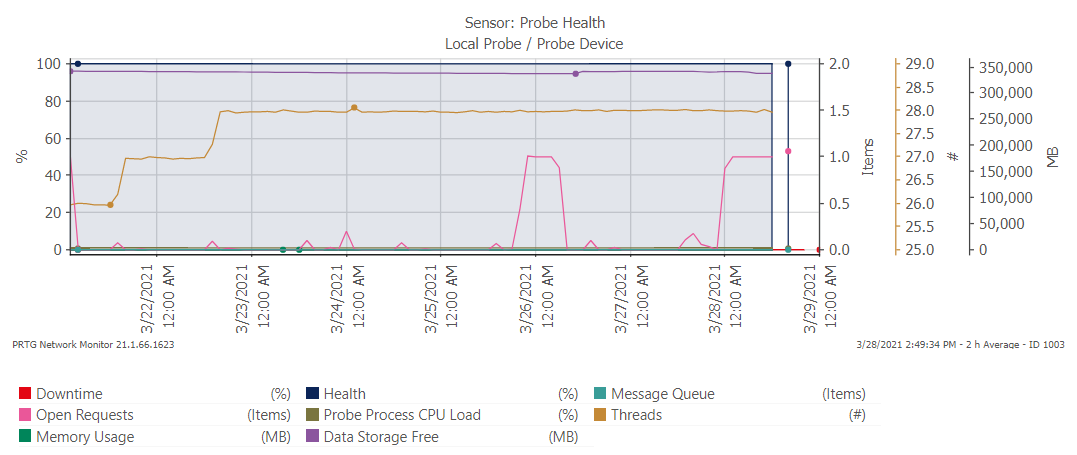
\includegraphics[width=\linewidth]{probe_health.png}
    \caption{Gráfico de 7 dias do sensor Probe Health gerado pelo PRTG.}
\end{figure}

O sensor \emph{Probe health} demonstra com detalhes métricas de funcionamento do \emph{probe device} em relação ao PRTG, como downtime, uso de memória (pelo PRTG), número de threads e CPU load. Observando a medição realizada durante os 7 dias, percebe-se que com o computador em funcionamento por mais tempo o número de threads tende a subir no começo mas estabilizar-se após um ou dois dias. Também foram verificados dois picos de requisições em aberto, durante duas madrugadas, provavelmente ocasionado pelas sessões de jogos online realizadas durante esse período.

\subsection{System health}

\begin{figure}[H]
    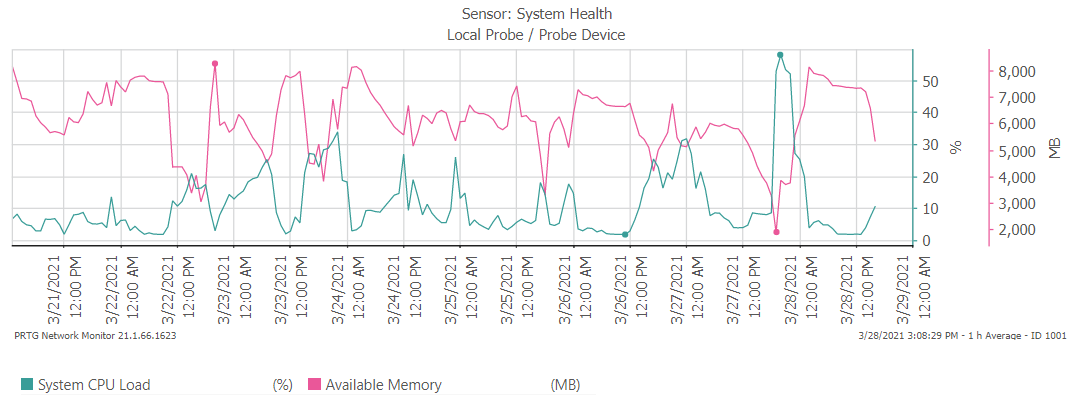
\includegraphics[width=\linewidth]{system_health.png}
    \caption{Gráfico de 7 dias do sensor System Health gerado pelo PRTG.}
\end{figure}

O sensor \emph{System health} monitora o hardware sistema hospedeiro, a fim de verificar picos de uso do sistema e as causas deles. Na medição realizada podemos ver que a máquina em questão está sempre com grandes quantidades de carga, isso se deve ao sistema Windows utilizar RAM proporcional a RAM disponível, além disso a máquina também roda serviços como o PostgreSQL e MongoDB que ficam ligados durante todo o dia consumindo recursos.

\subsection{Common SaSS Check}

\begin{figure}[H]
    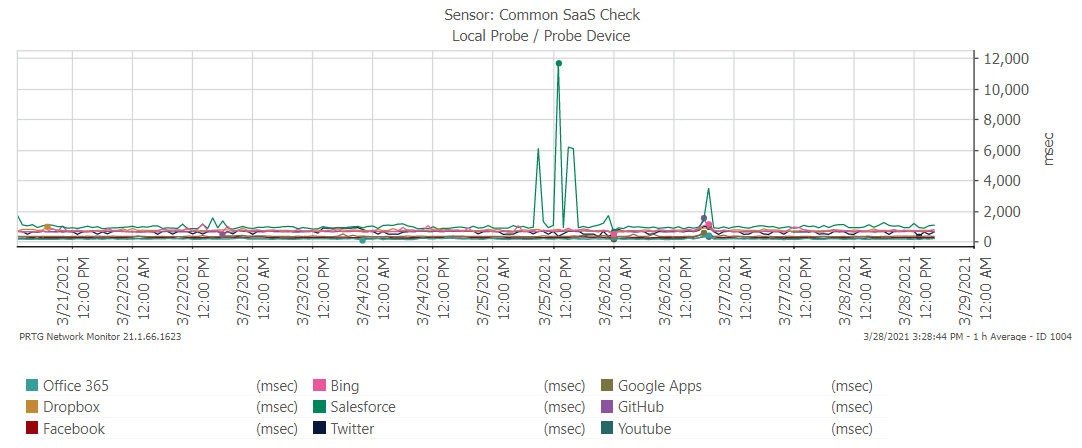
\includegraphics[width=\linewidth]{sass_check.png}
    \caption{Gráfico de 7 dias do sensor Common SaSS Check gerado pelo PRTG.}
\end{figure}

Esse sensor verifica a disponibilidade (em forma de ping) de serviços online comuns a serem utilizados em um escritório, pode ser muito útil no gerenciamento de uma rede corporativa. Durante a maior parte dos serviços se manteve abaixo de 300ms, mas podemos destacar um pico de mais de 11k de milissegundos no serviço da Salesforce, ocorrido no dia 25 de março entre 12:00PM e 01:00PM, provavelmente algum problema no próprio serviço da salesforce, considerando que os outros serviços não demonstraram esse pico.

\subsection{HTTP}

\begin{figure}[H]
    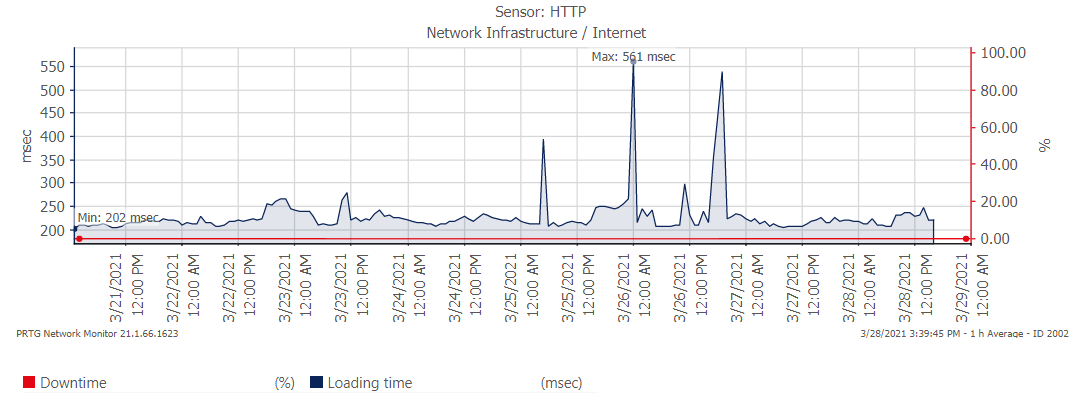
\includegraphics[width=\linewidth]{http.png}
    \caption{Gráfico de 7 dias do sensor HTTP gerado pelo PRTG.}
\end{figure}

O sensor HTTP monitora tempo de carregamento de páginas através do protocolo de comunicação HTTP, muito utilizado em browsers para acessar sites. No monitoramento foi verificado um pico acima de 500 ms, ao olhar no histórico de navegação foi possível constatar que nesse horário o único site sendo carregado era o twitter.com.

\subsection{Ping - Network device}

\begin{figure}[H]
    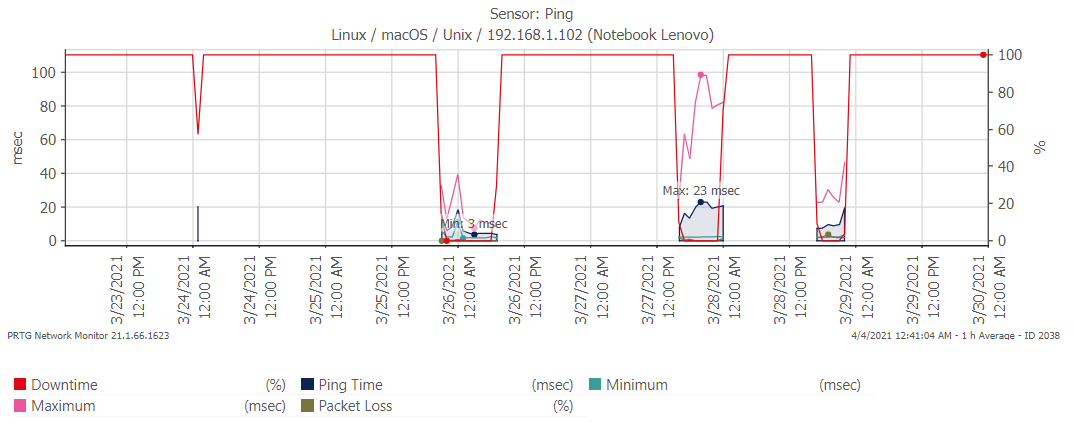
\includegraphics[width=\linewidth]{ping_notebook.png}
    \caption{Gráfico de 7 dias do sensor ping gerado pelo PRTG.}
\end{figure}

O sensor de ping monitora o tempo de resposta um ping pelo protocolo TCP/IP, o PRTG permite monitorar pings para quaisquer dispostivos da rede, no monitoramento foi abaixo foram realizados pings para o Notebook Lenovo citado na sessão de topologia de rede. O tempo de monitoramento nele foi menor pois o notebook em questão não fica ligado durante o tempo todo como o Desktop utilizado de \emph{probe device}.

\section{Wireshark}

\subsection{Address Resolution Protocol (ARP)}

O Address Resolution Protocol (ARP) transforma endereços da camada da internet (normalmente um endereço IPV4) em endereços da camada de enlace (como por exemplo um endereço MAC), esse protocolo é essencial para o funcionamento da internet e de redes locais. No Wireshark podemos monitorar o funcionamento do protocolo ARP por meio de um filtro, já que o software tem em sua configuração padrão a capacidade de monitorar o protocolo.

A imagem abaixo foi obtida após um monitoramento de 5 minutos contínuos no Wireshark, com o filtro \emph{arp} ligado (dessa forma o software ignora todos os outros protocolos e comunicações). Podemos perceber que o dispositivo com endereço 192.168.1.100 (Desktop) envia pela rede um pedido de identificação das máquinas com endereço 192.168.1.101 (Macbook) e 192.168.1.102 (Notebook Lenovo). O dispositivo com endereço 192.168.1.101 responde, enviando seu endereço MAC como identificação. O dispositivo com endereço 192.168.1.102 não envia resposta, então o Desktop continua fazendo pedidos pela rede. Também vemos uma troca de mensagens entre o Desktop e o roteador TPLink, quando o Desktop pergunta ao roteador qual seu endereço MAC.

\begin{figure}[H]
    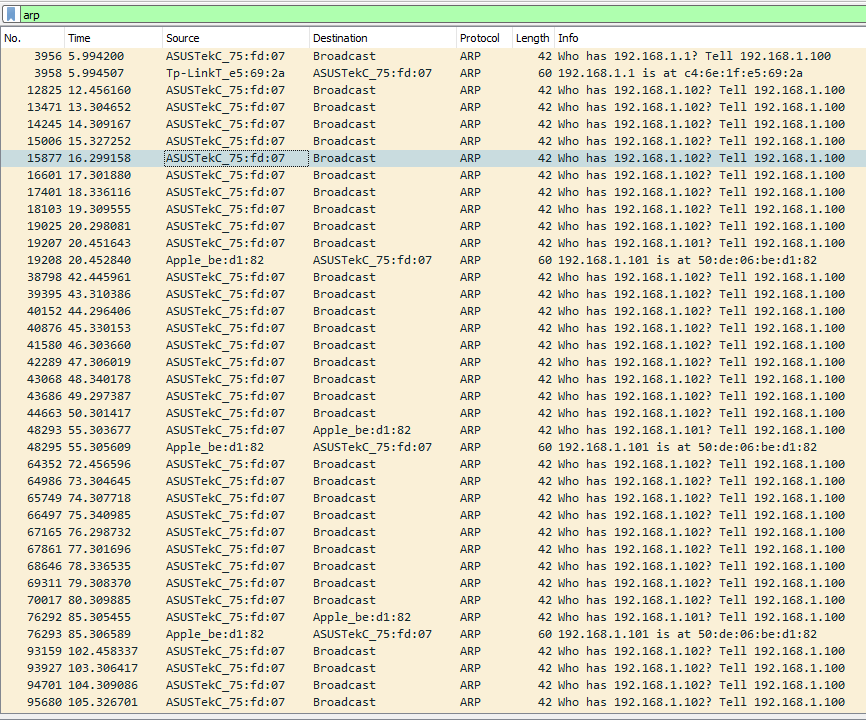
\includegraphics[width=\linewidth]{wireshark_arp.png}
    \caption{Tabela de ocorrências do protocolo ARP monitoradas pelo Wireshark.}
\end{figure}

\subsection{Simple Network Management Protocol (SNMP)}

Simple Network Management Protocol é um protocolo para organização de dispositivos gerenciados em uma rede IP, o Wireshark também é capaz de captar nativamente as trocas de mensagens relativas ao SNMP, por meio do filtro \emph{snmp} podemos configurar o software para mostrar apenas essas mensagens.

Na imagem abaixo foi realizado um monitoramento por mais de uma hora a fim de capturar mensagens relativas ao SNMP, o monitoramento se extendeu tanto devido a uma demora na captação de mensagens do tipo. Todas as transmissões interceptadas foram realizadas pelo dispositivo de IP 192.168.1.100 (Desktop) com o destino sendo o dispositivo de IP 192.168.137.9 que é um adaptador Wireless conectado a outra máquina. Todas as transmissões são do tipo \emph{get-next-request} 

\begin{figure}[H]
    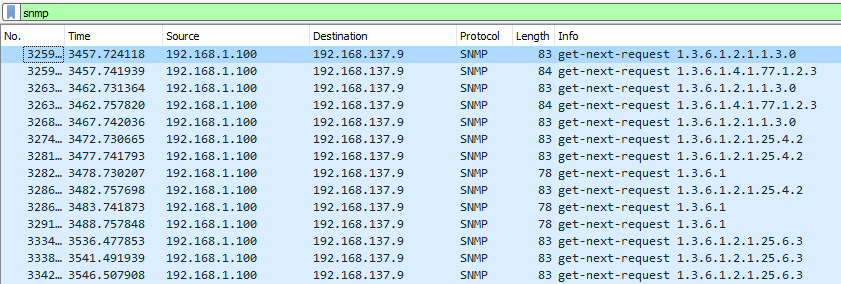
\includegraphics[width=\linewidth]{wireshark_snmp.png}
    \caption{Tabela de ocorrências do protocolo SNMP monitoradas pelo Wireshark.}
\end{figure}

\section{Conclusão}

Para realizar o presente trabalho foi necessário pesquisar e entender o funcionamento de ferramentas utilizadas na gerência de redes, como o PRTG e o Zabbix. Utilizando essa ferramenta podemos perceber o funcionamento de uma rede doméstica em suas nuances mais específicas, podendo utilizar esses conhecimentos para otimizar a rede e os processos envolvidos em um futuro trabalho profissional.

Para utilizar o Wireshark para compreender o tráfego geral da rede também foi necessário estudar e compreender o funcionamento de protocolos como ARP, SNMP, TCP, UDP e outros, a fim de analisar com mais precisão o output gerado pelo programa. Essa etapa se mostrou fundamental para a análise geral da rede. Com tudo isso dito, fica evidente a importância desse trabalho na agregação de conhecimento ao aluno que o desenvolve com comprometimento e seriedade, sendo um bom marco na formação do estudante de ciência da computação.

\nocite{*}
\medskip

\bibliographystyle{abbrv}
\bibliography{biblio}

\end{document}